\chapter{Concept and Design}
\label{chapter:concept}


\section{Blockchain Technology}

The blockchain market as of the time of writing is not totally rough out. In the last years two main services stood out in particular, \textit{Bitcoin} \citep{BitcoinMainPage} and \textit{Ethereum} \citep{EthereumMainPage}.

\subsection{Bitcoin}

\textbf{Non Touring complete} https://en.bitcoin.it/wiki/Script


\subsection{Ethereum}
Ethereum is a decentralized platform for the creation an publication peer-to-peer of \textit{smart contracts}.
It ran out in \textit{live} mode for the first time on July 2015 \citep{EthereumLaunch}, and since then it received a strong consensus from the community in the last months \citep{EthereumEuroChart}.

Unlike Bitcoin, Ethereum provide a Turing Complete language, allowing the user to create a most detailed and adaptable contracts.

\begin{figure}[ht]
  \vspace{2em}
	\centering
  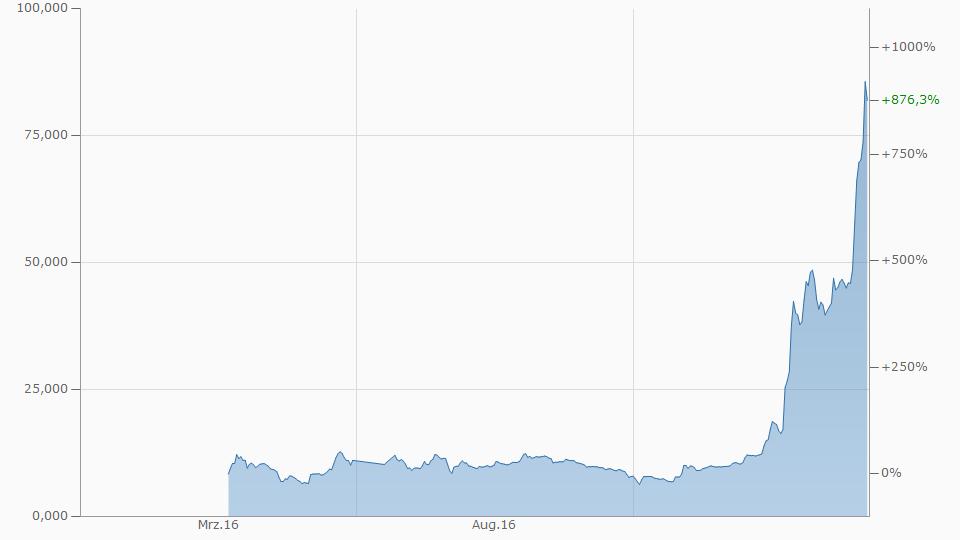
\includegraphics[width=0.8\linewidth]{ethereum-euro}
	\caption{Ethereum - Euro exchage chart}
	\label{fig1}
\end{figure}
